\section{Schritt für Schritt Anleitung}
\label{sec:StepbyStep}
Eine Schritt für Schritt Anleitung zum vollständigen Scannen und exportieren eines 3D-Objektes.


\begin{longtable}{|m{5cm}|m{8cm}|} 
\caption{Schritt für Schritt Anleitung}\\ \hline
\multicolumn{2}{|l|}{{\textbf{\label{tab:T_StepbyStep}Schritt 1 - Einschalten der Schrittmotorsteuerung}}}
\\ \hline
Auf der Rückseite des 19''-Rack befindet sich ein Schalter. Mit diesem kann die Steuerung eingeschaltet werden.
& 
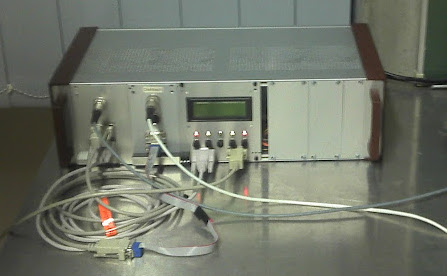
\includegraphics[width=8cm]{19Zoll_Rack}
\\ \hline 

\multicolumn{2}{|l|}{{\textbf{Schritt 2 - Einschalten des VI-900}}}\\ \hline
\multicolumn{2}{|p{13cm}|}{Bevor der VI-900 eingeschaltet wird, muss der Erfassungs-PC eingeschaltet werden. Kurz nach dem BIOS wird nach SCSI Geräten gesucht. Zu diesem Zeitpunkt muss der VI-900 eingeschaltet werden.}
\\ \hline 
 
\multicolumn{2}{|l|}{{\textbf{Schritt 3 - Einloggen}}}
\\ \hline
\multicolumn{2}{|l|}{{Der Benutzername lautet \textbf{Minolta}, das Passwort kann leer bleiben.}}
\\ \hline  
 
\multicolumn{2}{|l|}%
{{\textbf{Schritt 4 - Starten von RapidForm2004}}}
\\ \hline
Auf dem Desktop doppelt auf das Icon \textbf{RapidForm} klicken.
& 
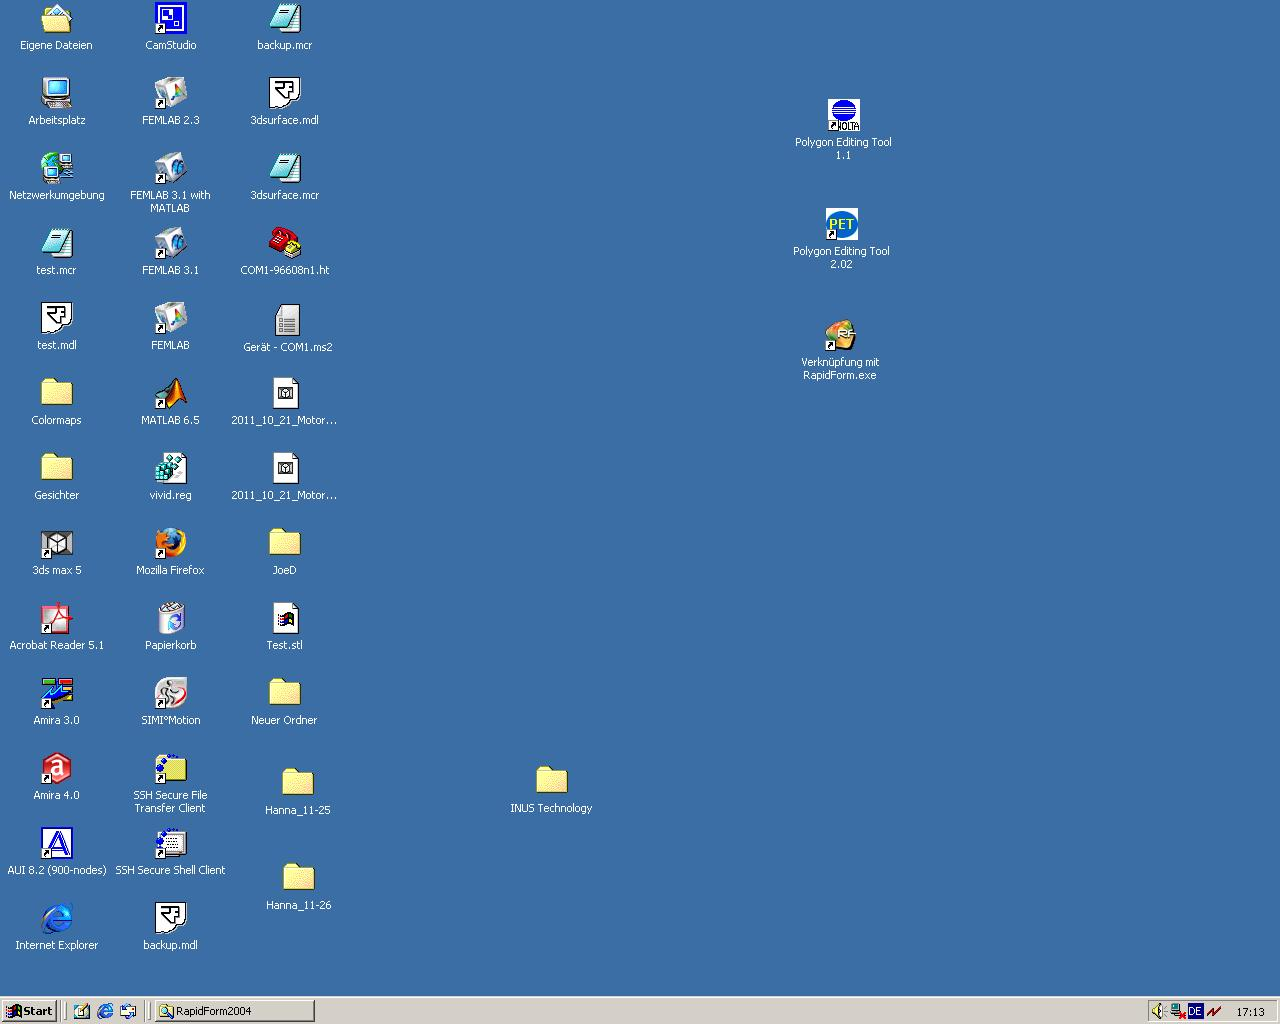
\includegraphics[width=8cm]{Anleitung/1_Desktop}
\\ \hline 
\newpage
\multicolumn{2}{|l|}%
{{\textbf{Schritt 5 - Oberfläche von RapidForm2004}}}
\\ \hline
Die Oberfläche unterteilt sich in Menü, Werkzeugleisten, Projektbaum und Anzeigefläche.
Je nach dem welche Ansicht in der Anzeigefläche gewählt ist, verändern sich auch das Menü und die Werkzeugleisten. 
& 
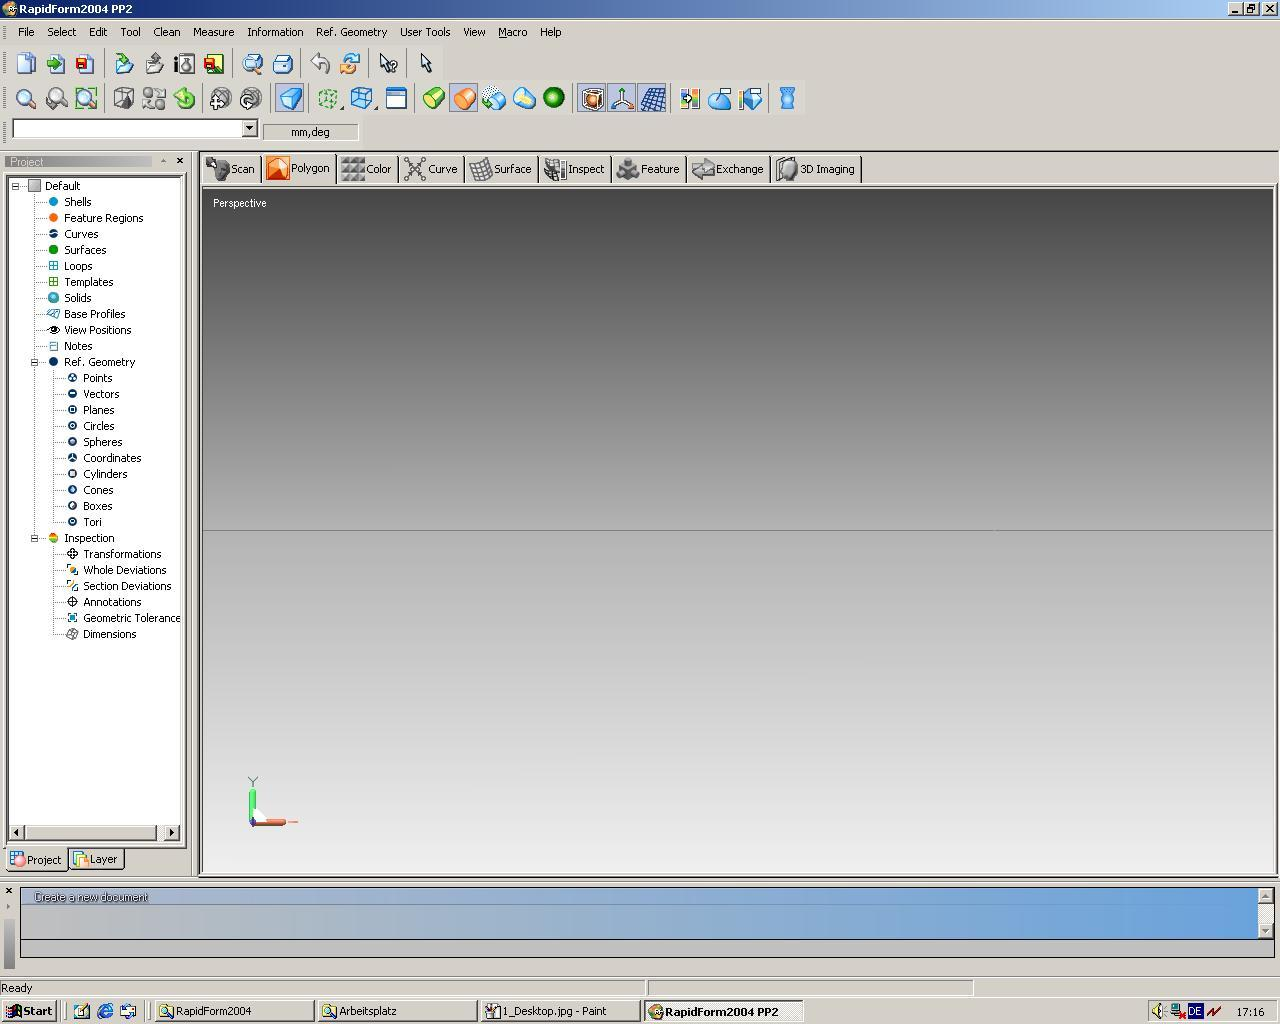
\includegraphics[width=8cm]{Anleitung/2_RapidForm}
\\ \hline  

\multicolumn{2}{|l|}%
{{\textbf{Schritt 6 - Starten des ''ADD-IN''}}}
\\ \hline
In der Menüzeile auf 
\textbf{Macro -> Addins -> Konica Minolta VIVID Direct Control Addin v2.6.11}
klicken.
& 
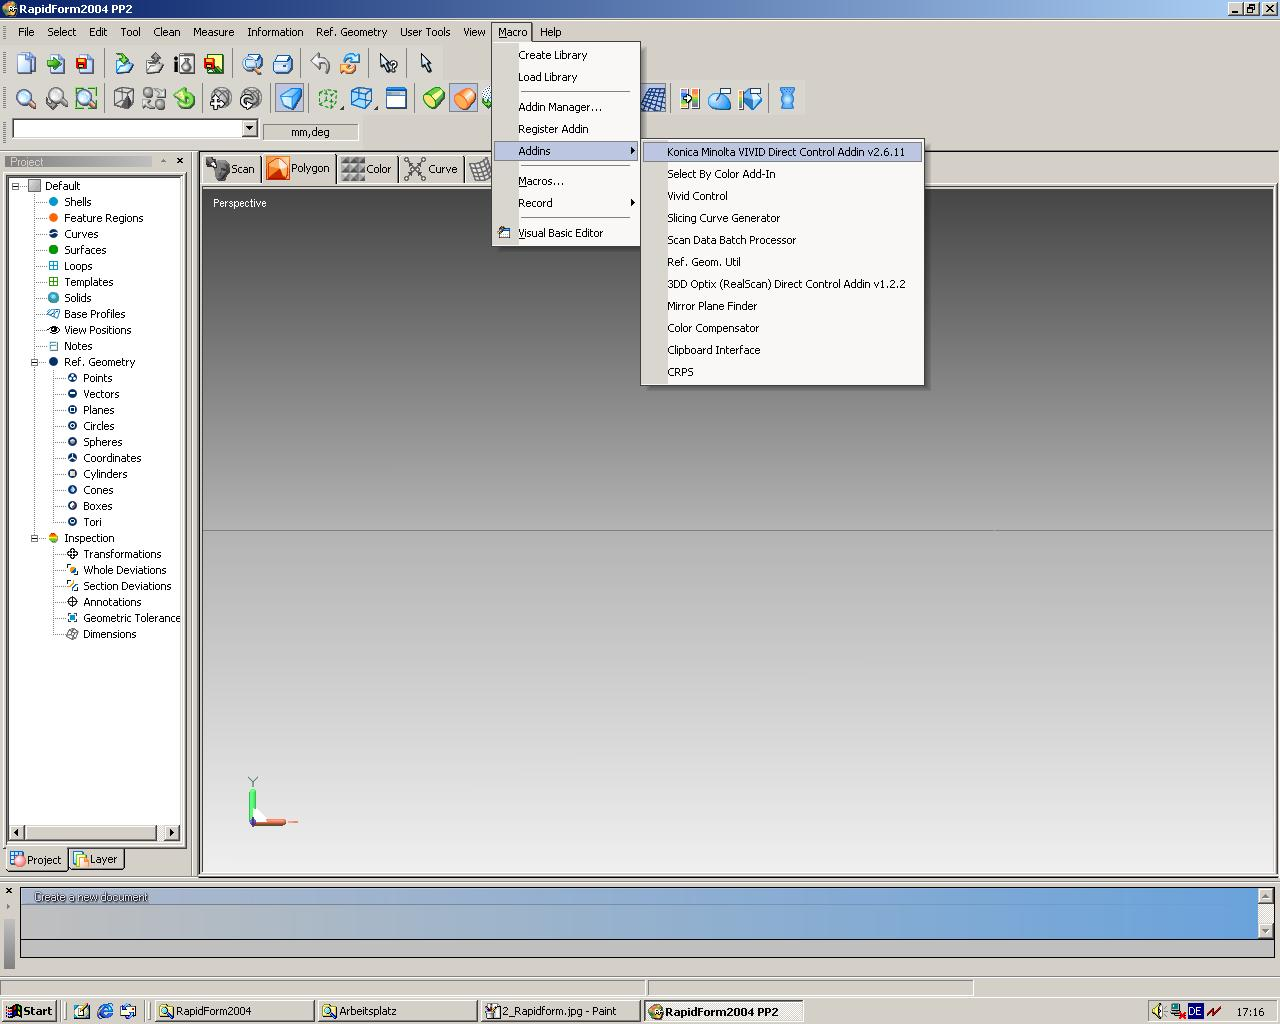
\includegraphics[width=8cm]{Anleitung/3_ADDIN_Menu}
\\ \hline  

\pagebreak

\multicolumn{2}{|l|}%
{{\textbf{Schritt 7 - Verbinden des Schrittmotor}}}
\\ \hline
Damit der Drehtisch genutzt werden kann muss dieser im Add-In ausgewählt werden. Dazu im unteren Bereich den Reiter \textbf{Rotary Table} auswählen. Dort aus dem Dropdown Menü den Drehtisch \textbf{ISEL RF-1} auswählen. Die Befehle für diesen Drehtisch werden vom Mikrocontroller am besten unterstützt.
Anschließend auf \textbf{Connect} klicken.\linebreak
Bei einem Fehler überprüfen ob die Steuerung eingeschaltet ist und alle Verbindungen hergestellt wurden.
& 
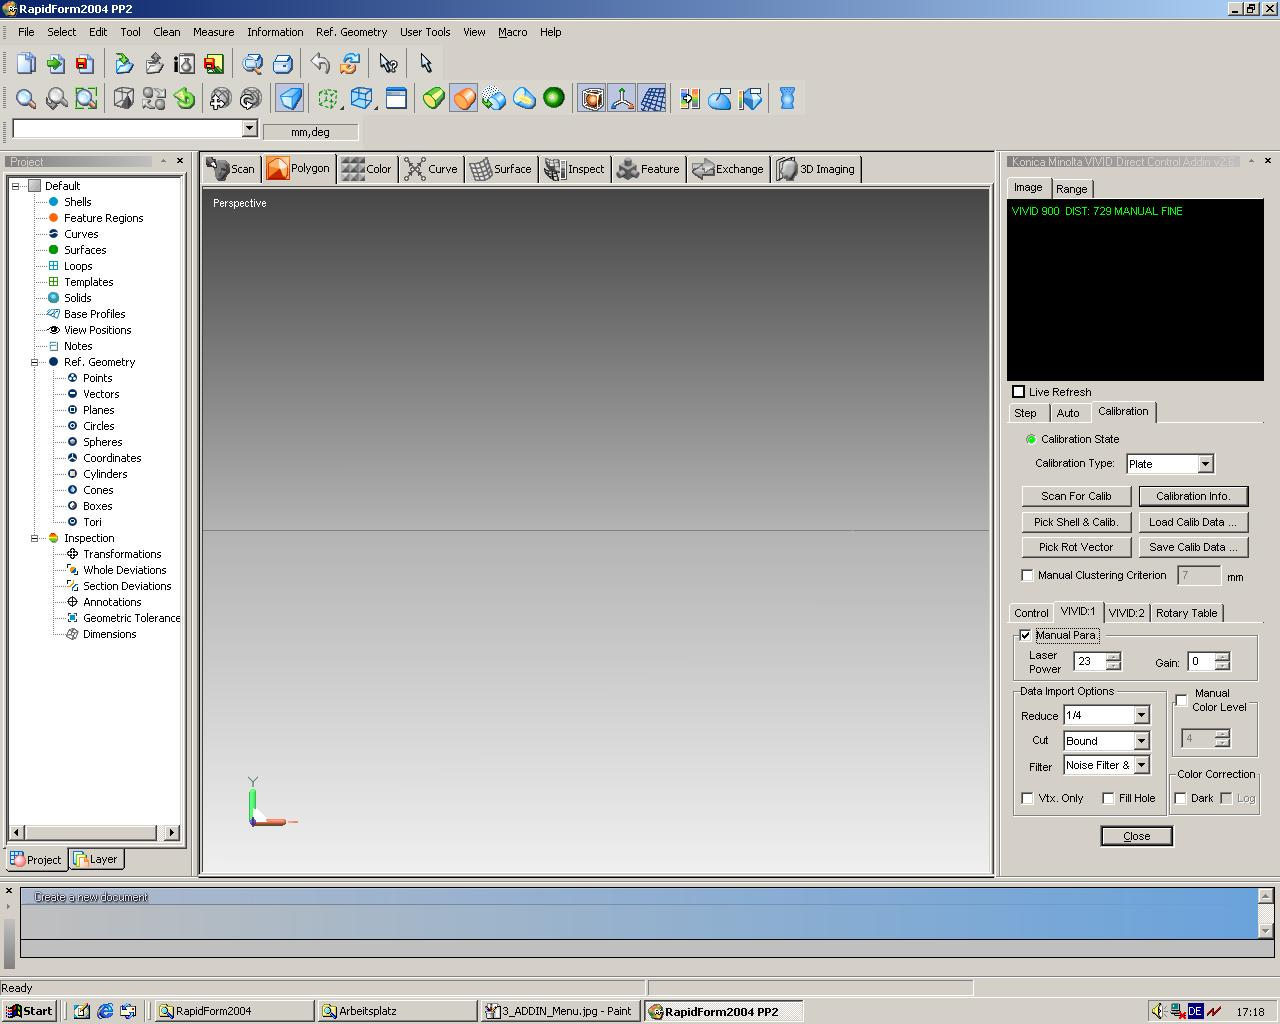
\includegraphics[width=8cm]{Anleitung/4_Calibration}
\\ \hline  

\multicolumn{2}{|l|}%
{{\textbf{Schritt 8 - Kalibrieren vorbereiten}}}
\\ \hline
%\begin{TippS}
Für ein erfolgreiches Zusammenführen der einzelnen Aufnahmen ist die Kalibrierung unerlässlich!
%\end{TippS}
Auf dem Add-In Panel, unter dem Vorschau Fenster, auf \textbf{Live-Preview} klicken. \linebreak
Das Kalibrierungsblech auf dem Drehtisch positionieren.  \linebreak
Dabei muss der Noppen an der Unterseite des Kalibrierungsblechs in das mittlere Loch des Drehtisches gesteckt werden. Die abgeklebte Seite muss zum VI-900 zeigen.
& 
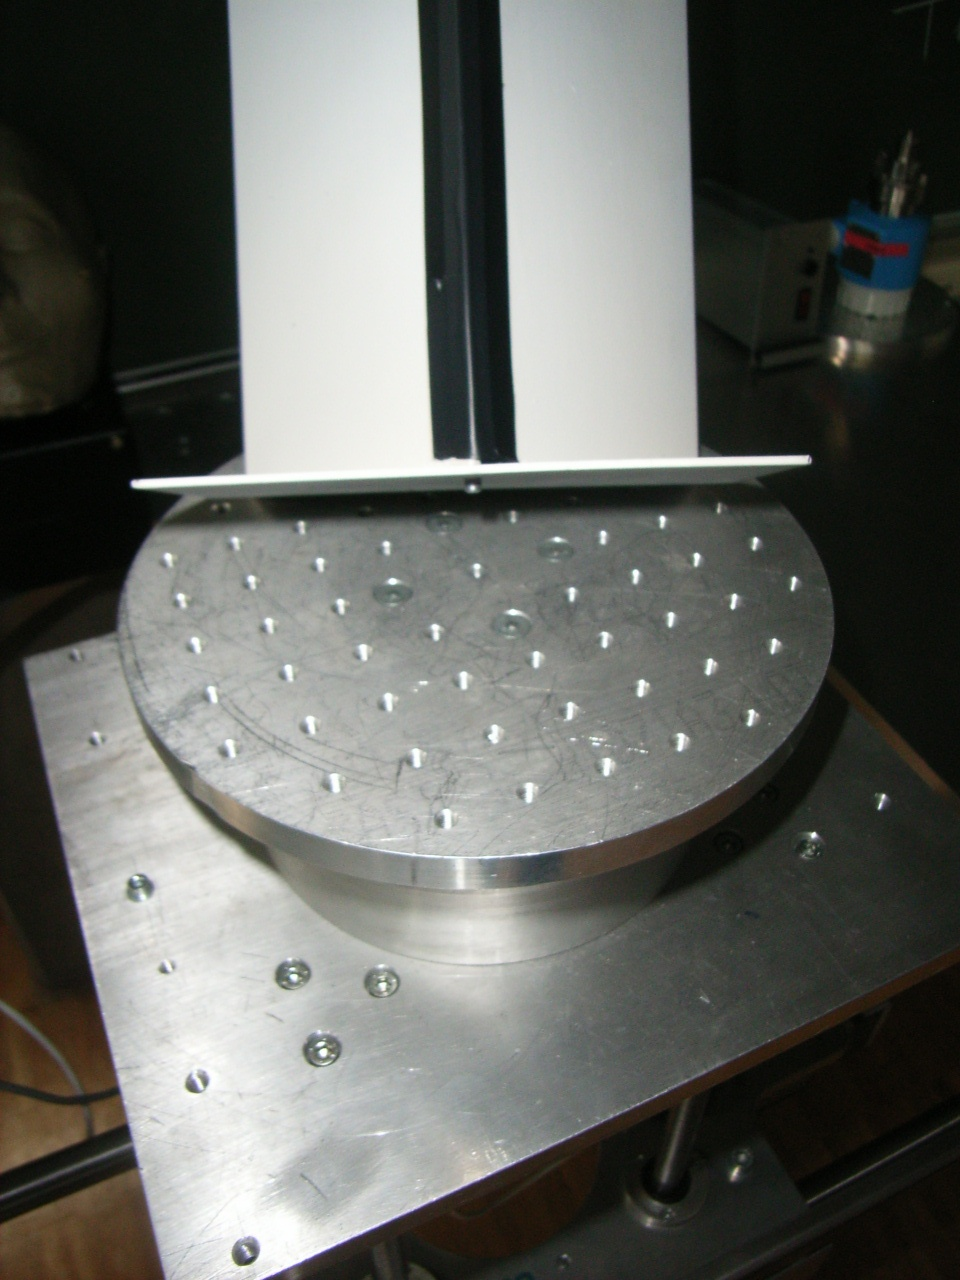
\includegraphics[width=8cm]{Anleitung/4_5_Calibration}
\\ \hline  

\pagebreak

\multicolumn{2}{|l|}%
{{\textbf{Schritt 9 - Kalibrieren}}}
\\ \hline
Den Reiter \textbf{VIVID: 1} auswählen.\linebreak
Bei \textbf{Manual Para.} ein Häkchen setzen.\linebreak
Im Feld \textbf{Laser Power} ''23'' eintragen.\linebreak
Auf \textbf{Scan for Calib} klicken.
& 
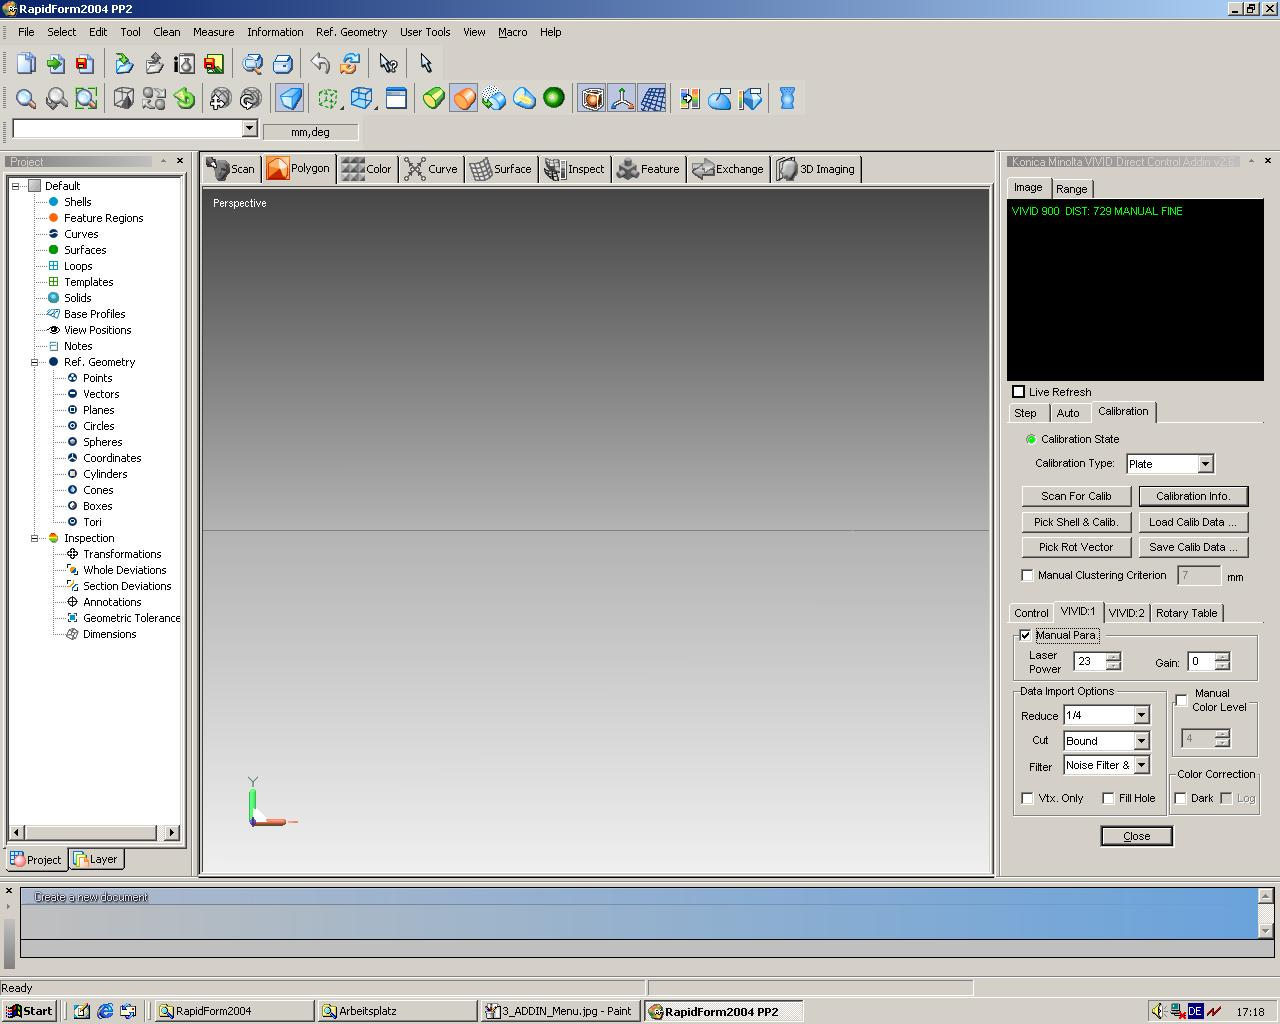
\includegraphics[width=8cm]{Anleitung/4_Calibration}
\\ \hline  

\multicolumn{2}{|l|}%
{{\textbf{Schritt 10 - Kalibrierungsergebnis}}}
\\ \hline
Das Ergebnis sollte ähnlich zu dem in der rechten Abbildung sein. \linebreak
Falls das Add-In einen Fehler ausgibt, muss das Kalibrierungsblech eventuell anders positioniert werden, der Wert im Feld \textbf{Laser Power} verändert werden oder der Fokus manuell eingestellt werden.\linebreak
War die Kalibrierung erfolgreich, können die \emph{Kalibrationsebenen} im \emph{Projektbaum} ausgeblendet werden.
& 
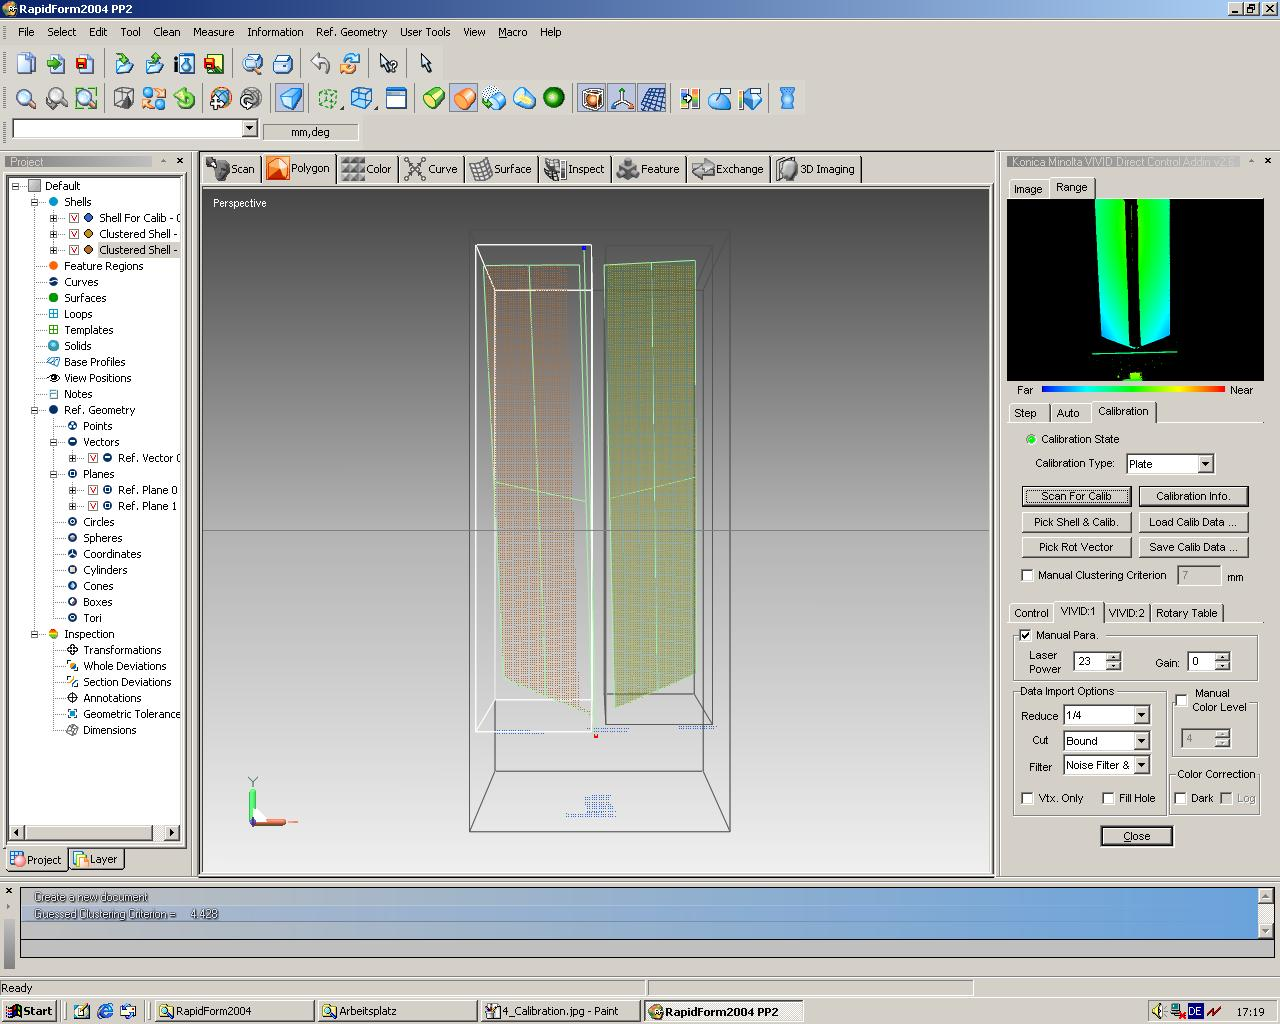
\includegraphics[width=8cm]{Anleitung/4_Calibration_result}
\\ \hline  

\pagebreak

\multicolumn{2}{|l|}%
{{\textbf{Schritt 11 - StepScan}}}
\\ \hline
Bei \textbf{Manual Para.} das Häkchen entfernen.\linebreak
Zum Reiter \textbf{Step} wechseln.\linebreak
Bei \textbf{Angle Tag} und \textbf{Rotate Table to next Scan position} Häkchen setzen.\linebreak
Bei \textbf{Init. Align in RF Using Rotary Info.} und \textbf{Auto Accept} die Häkchen entfernen.\linebreak
Bei \textbf{Rotation Step} die gewünschte Drehung in Grad eingeben. \linebreak
''45'', ''60'' und ''90'' sind gute Werte.
& 
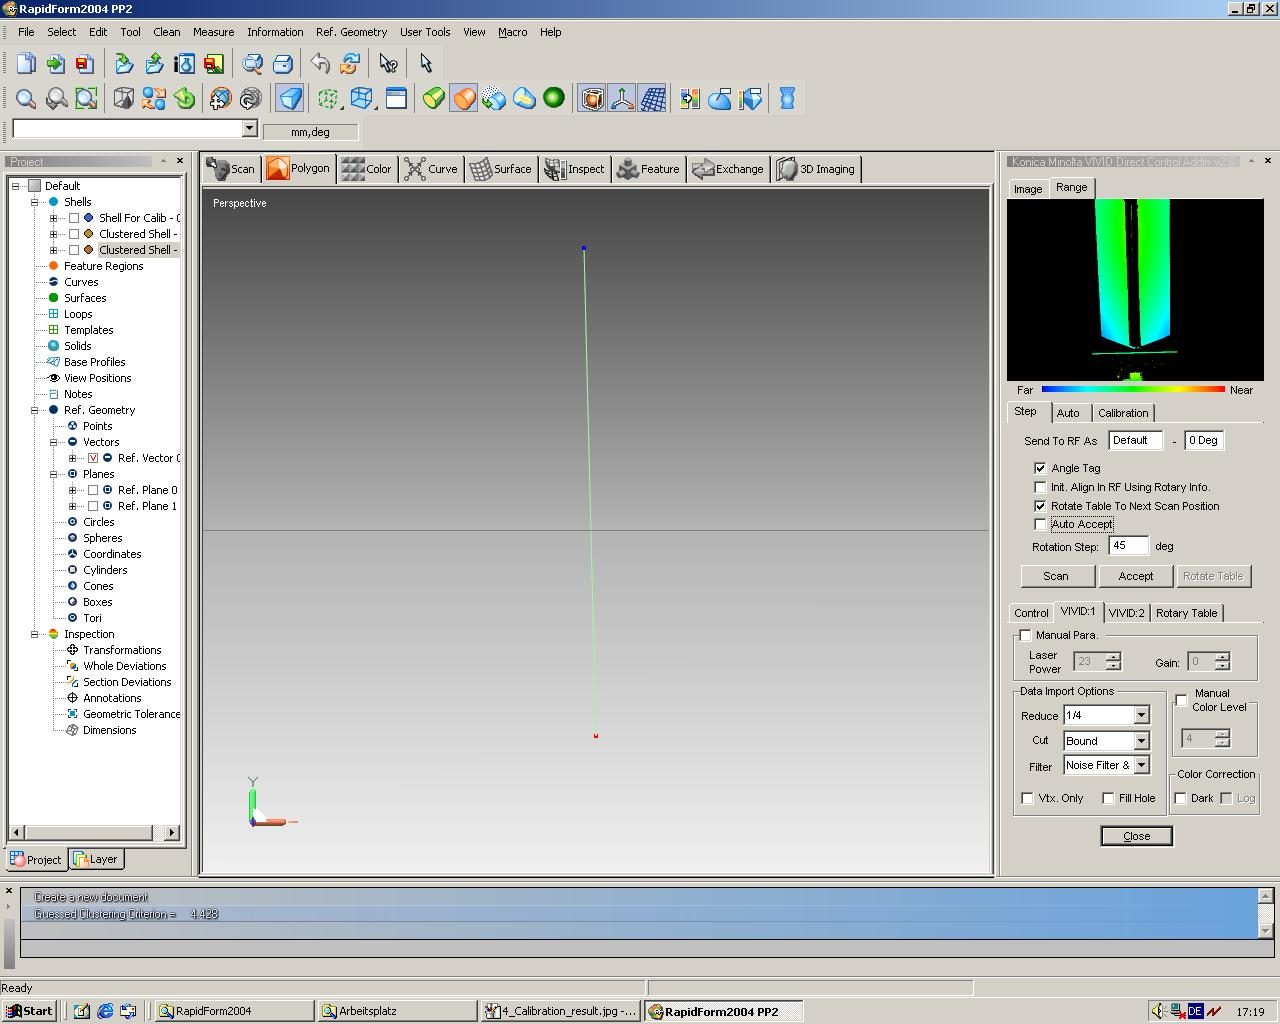
\includegraphics[width=8cm]{Anleitung/5_StepScan.jpg}
\\ \hline  

\multicolumn{2}{|l|}%
{{\textbf{Schritt 12 - AutoFocus}}}
\\ \hline
Das \emph{Kalibrationsblech} entfernen und durch das zu scannende Objekt ersetzen.\linebreak
Zum Reiter \textbf{Control} wechseln. \linebreak
Auf \textbf{Autofocus} klicken.\linebreak
& 
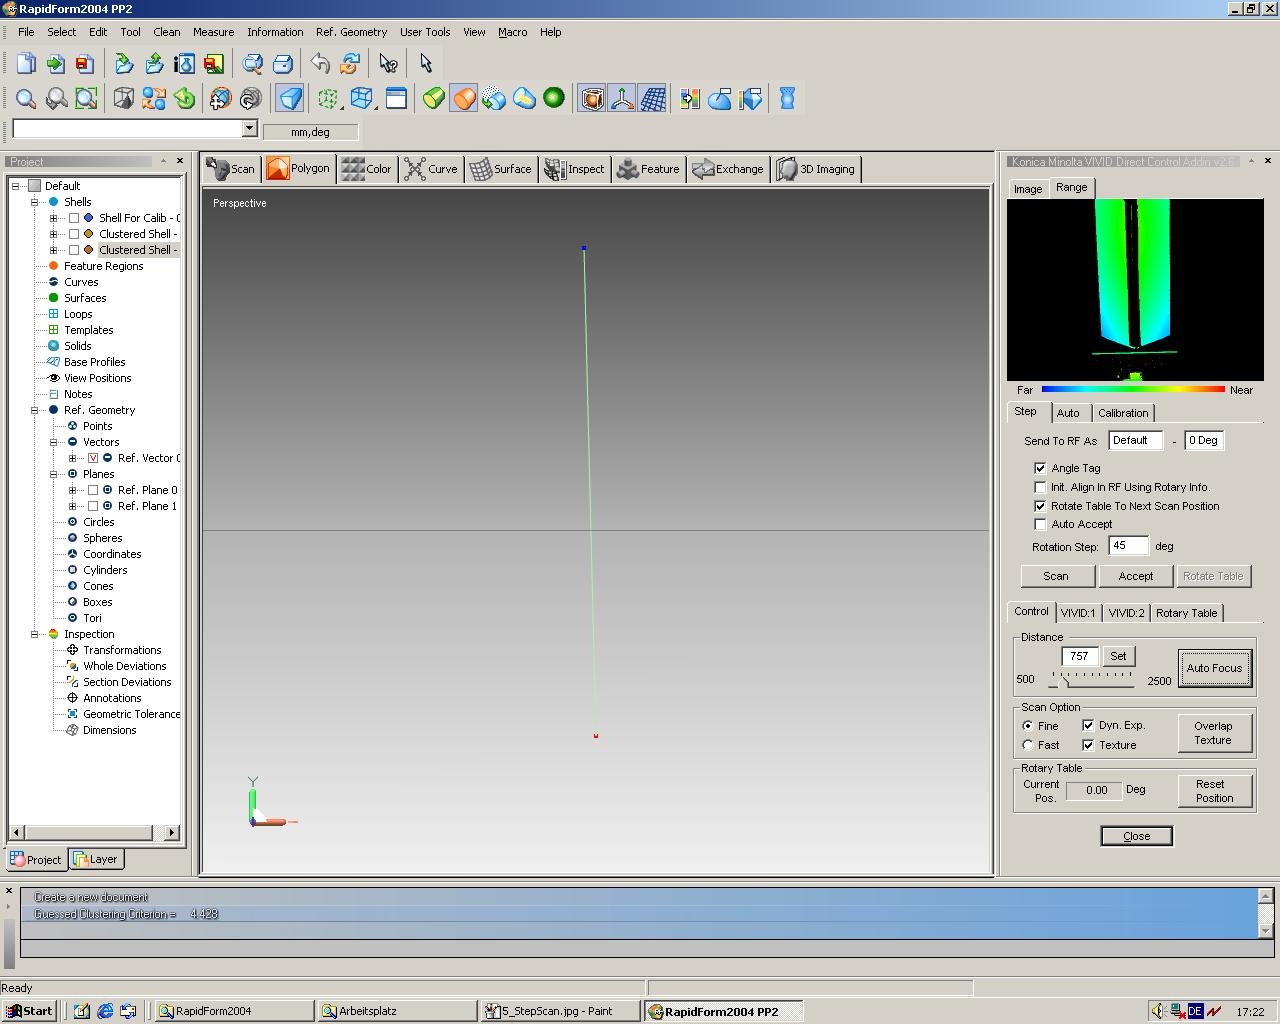
\includegraphics[width=8cm]{Anleitung/6_AutoFocus}
\\ \hline  

\pagebreak

\multicolumn{2}{|l|}%
{{\textbf{Schritt 13 - Scan}}}
\\ \hline
Auf \textbf{Scan} klicken. \linebreak
Das Objekt sollte möglichst schon zu erkennen sein und die Farben sich im Mittleren Bereich bewegen. \linebreak
Ansonsten muss mit den Parametern \textbf{Focus} und \textbf{LaserPower gespielt werden.}
%\begin{TippS}
Die Position des VI-900 darf nach der Kalibrierung nicht mehr verändert werden!
%\end{TippS}
& 
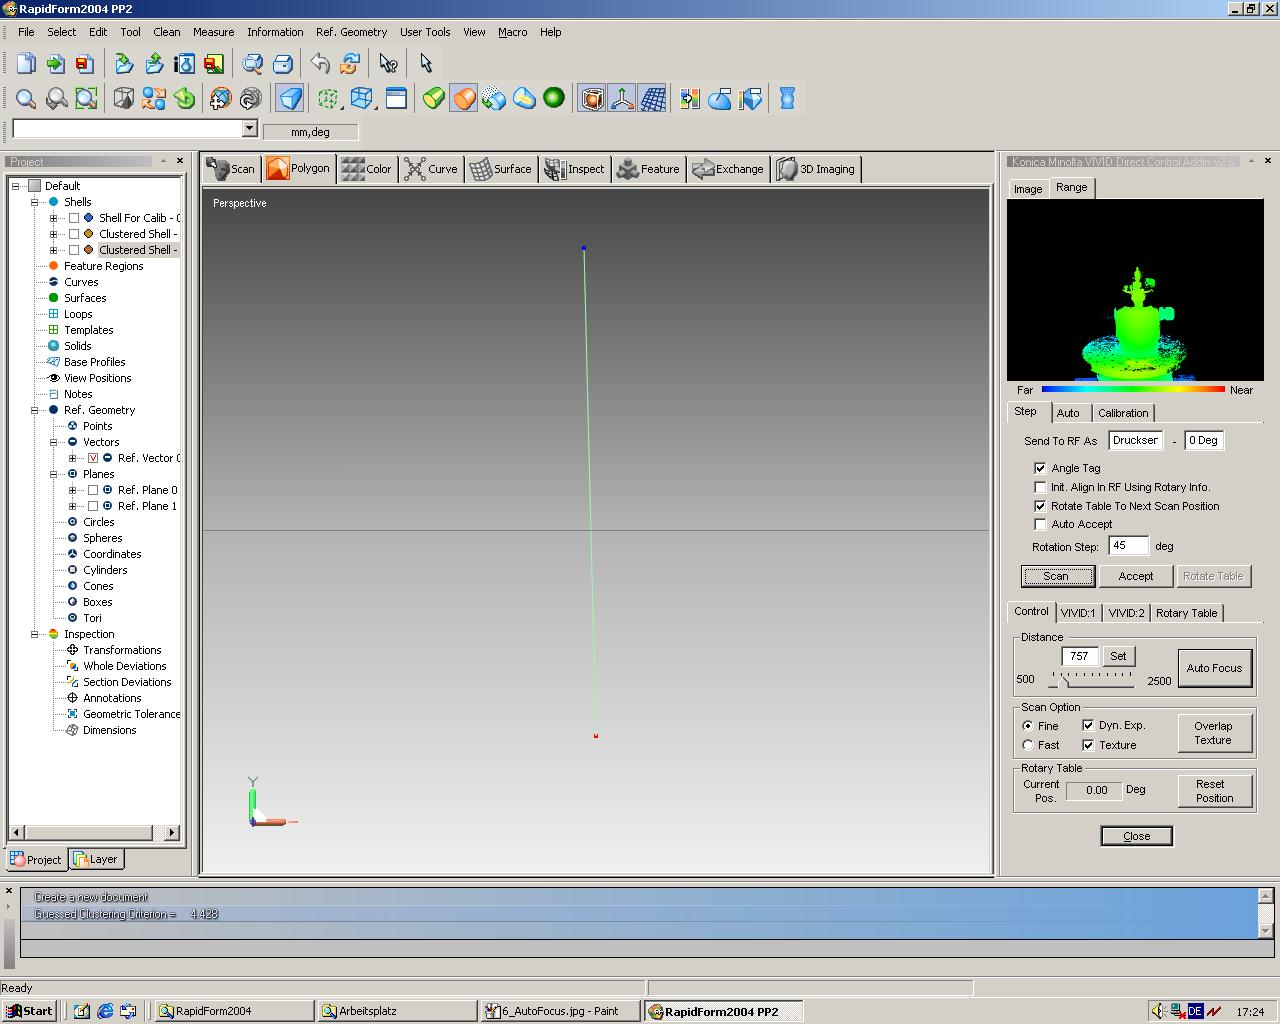
\includegraphics[width=8cm]{Anleitung/7_Scan}
\\ \hline  

\multicolumn{2}{|l|}%
{{\textbf{Schritt 14 - Akzeptieren}}}
\\ \hline
Ist das Objekt gut zu erkennen, können mit \textbf{Accept} die Daten an RapidForm2004 gesendet werden. Der Drehtisch sollte sich nun automatisch um den eingestellten Winkel drehen. 
%\begin{TippS}
Bei \textbf{AutoAccept} kann nun ein Häkchen gesetzt werden.
%\end{TippS}
& 
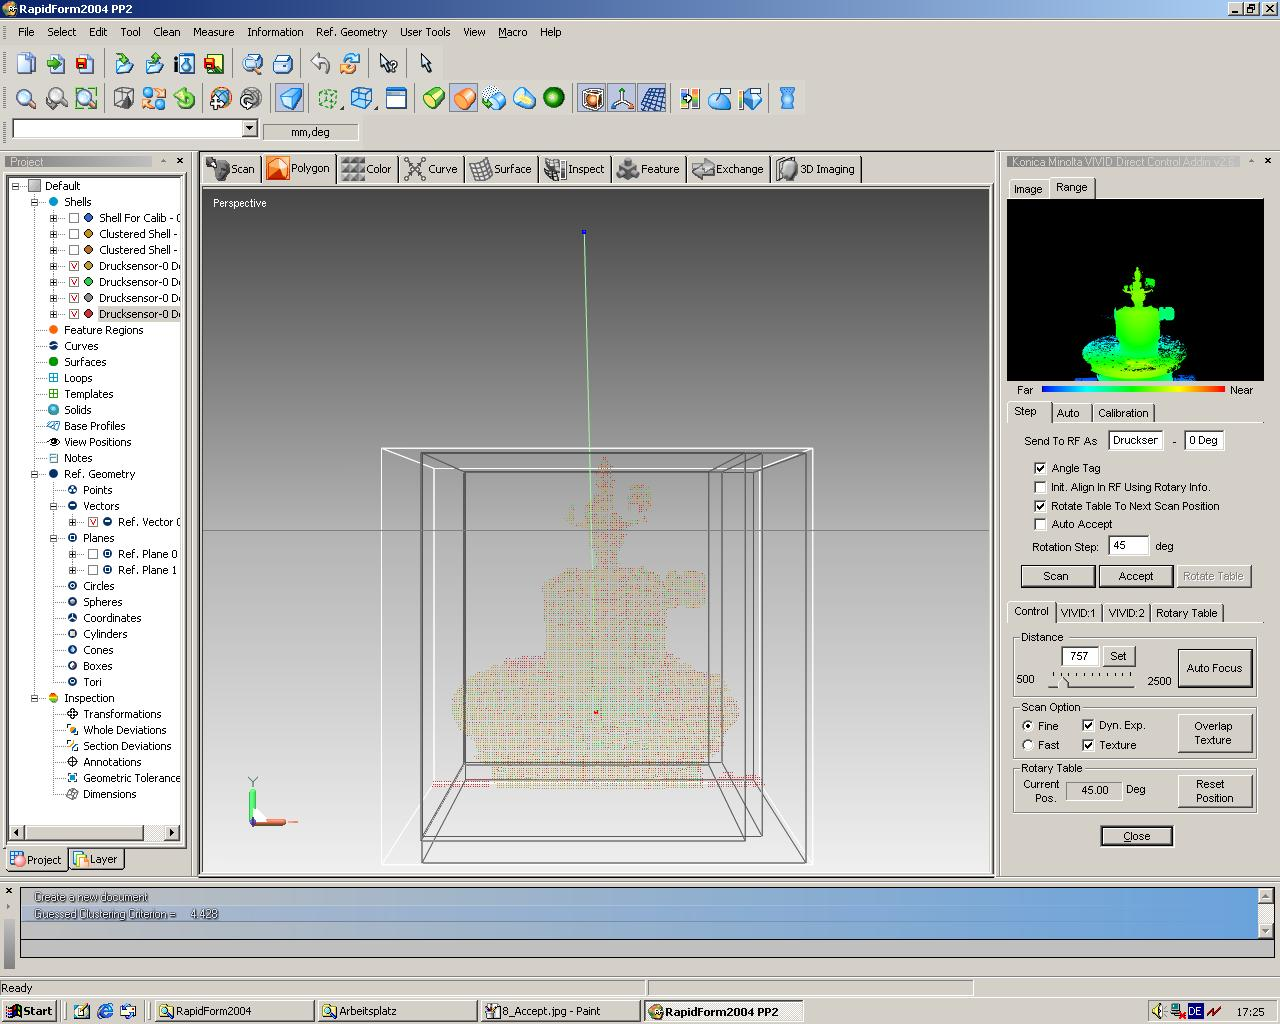
\includegraphics[width=8cm]{Anleitung/8_Accept}
\\ \hline  

\pagebreak

\multicolumn{2}{|l|}%
{{\textbf{Schritt 15 - Scannen}}}
\\ \hline
Auf \textbf{Scan} klicken und warten bis der Scan abgeschlossen ist und der Tisch sich gedreht hat.\linebreak
Diesen Schritt wiederholen bis alle Aufnahmen abgeschlossen sind.\linebreak
& 
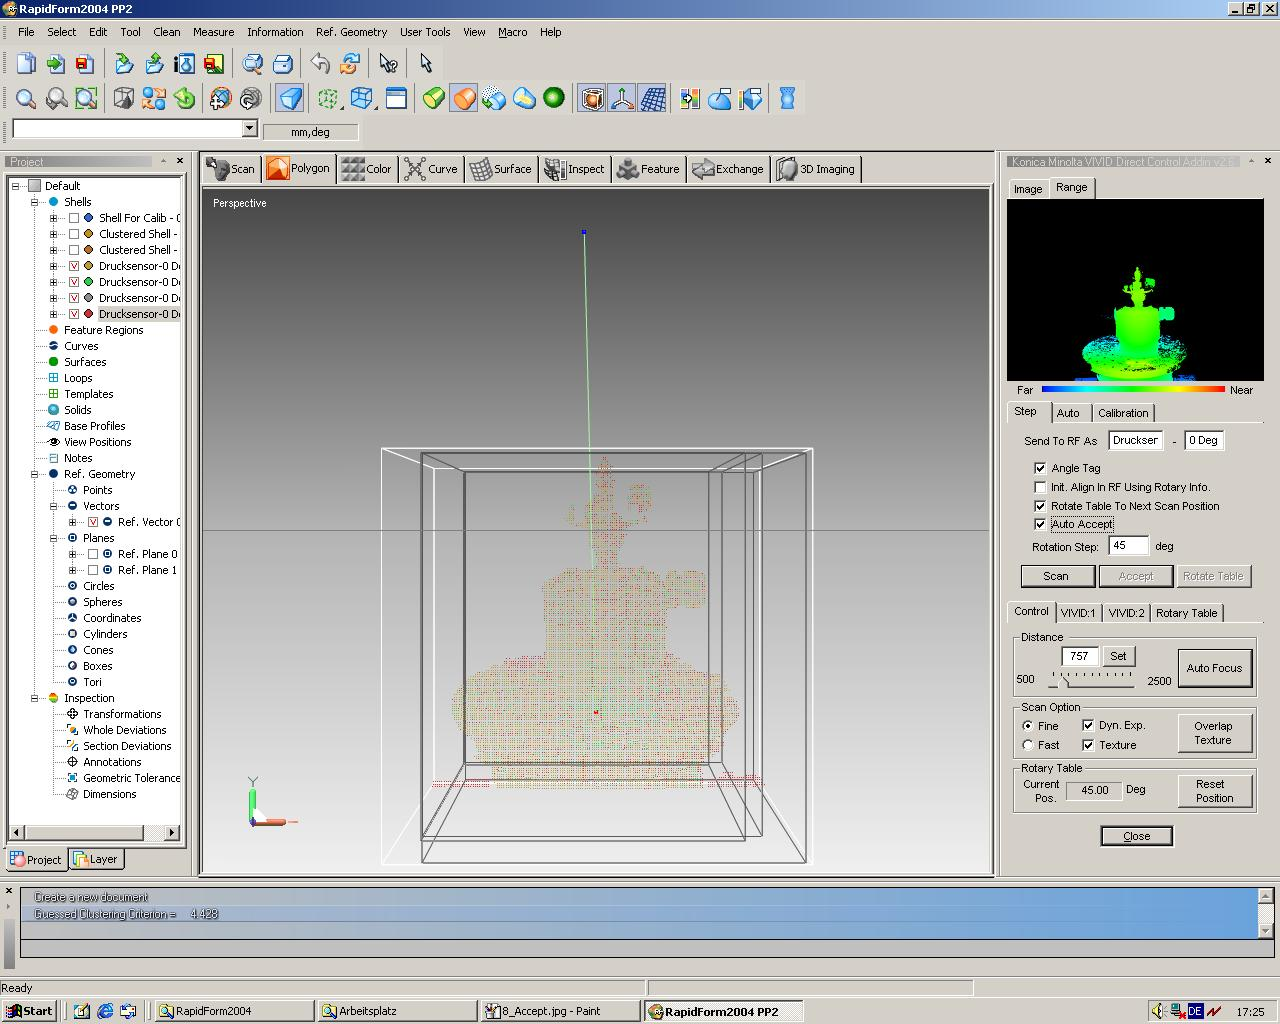
\includegraphics[width=8cm]{Anleitung/8_AutoAccept}
\\ \hline  

\multicolumn{2}{|l|}%
{{\textbf{Schritt 16 - Ergebnis der Scans}}}
\\ \hline
Nach Abschluss aller Scans dreht der Tisch sich automatisch in die Ursprungsposition zurück.\linebreak
Im Arbeitsbereich sollten sich nun alle Scans befinden.
& 
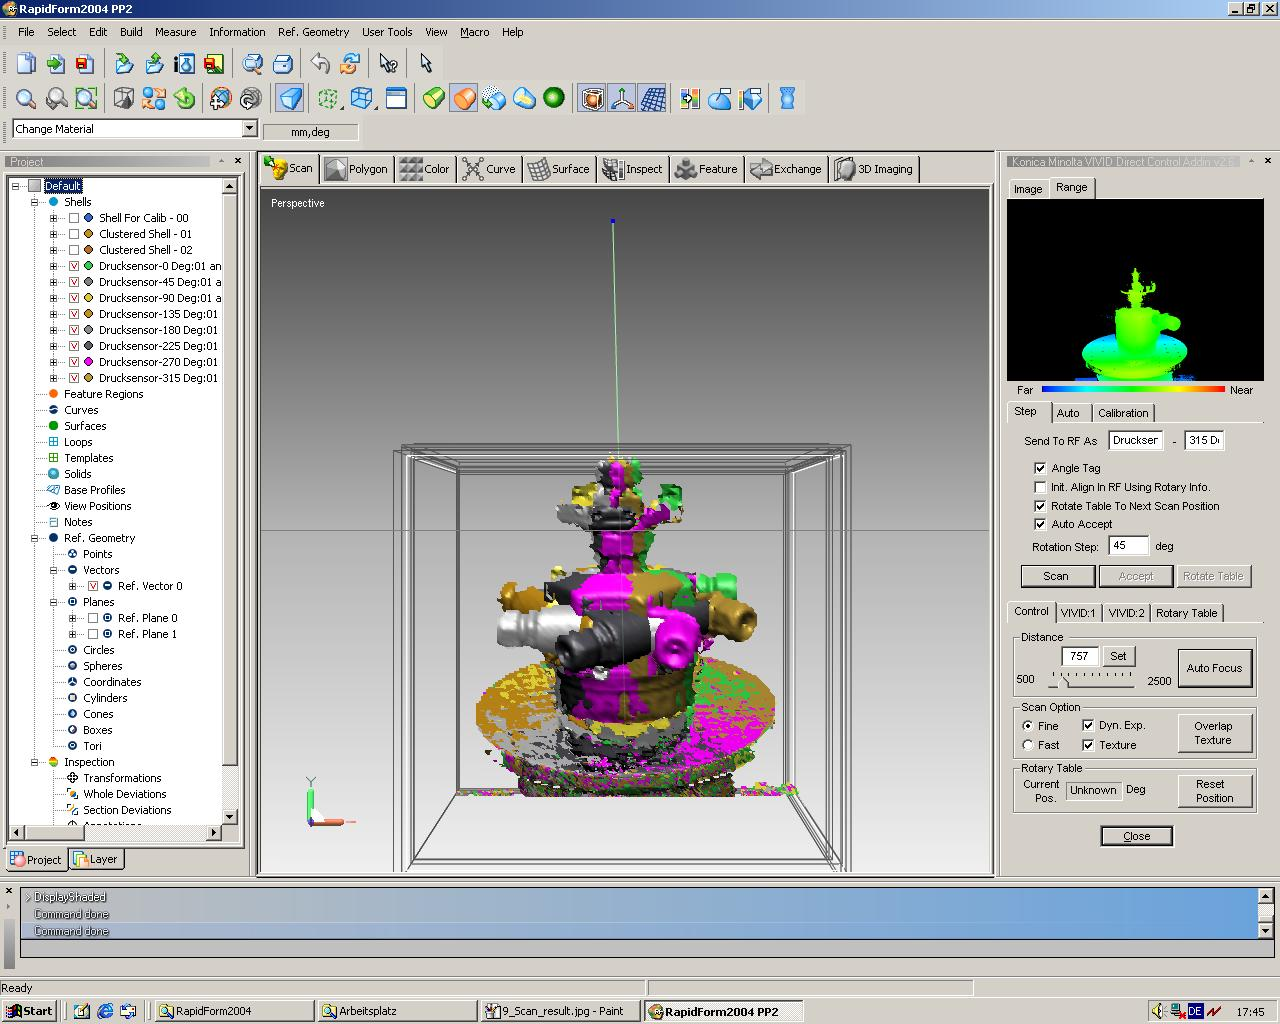
\includegraphics[width=8cm]{Anleitung/9_1_Scan_result}
\\ \hline  

\pagebreak

\multicolumn{2}{|l|}%
{{\textbf{Schritt 17 - Drehen und Zusammenführen der Scans}}}
\\ \hline
In der Menüzeile auf \textbf{Build -> Register -> Rotary Table} klicken.\linebreak
& 
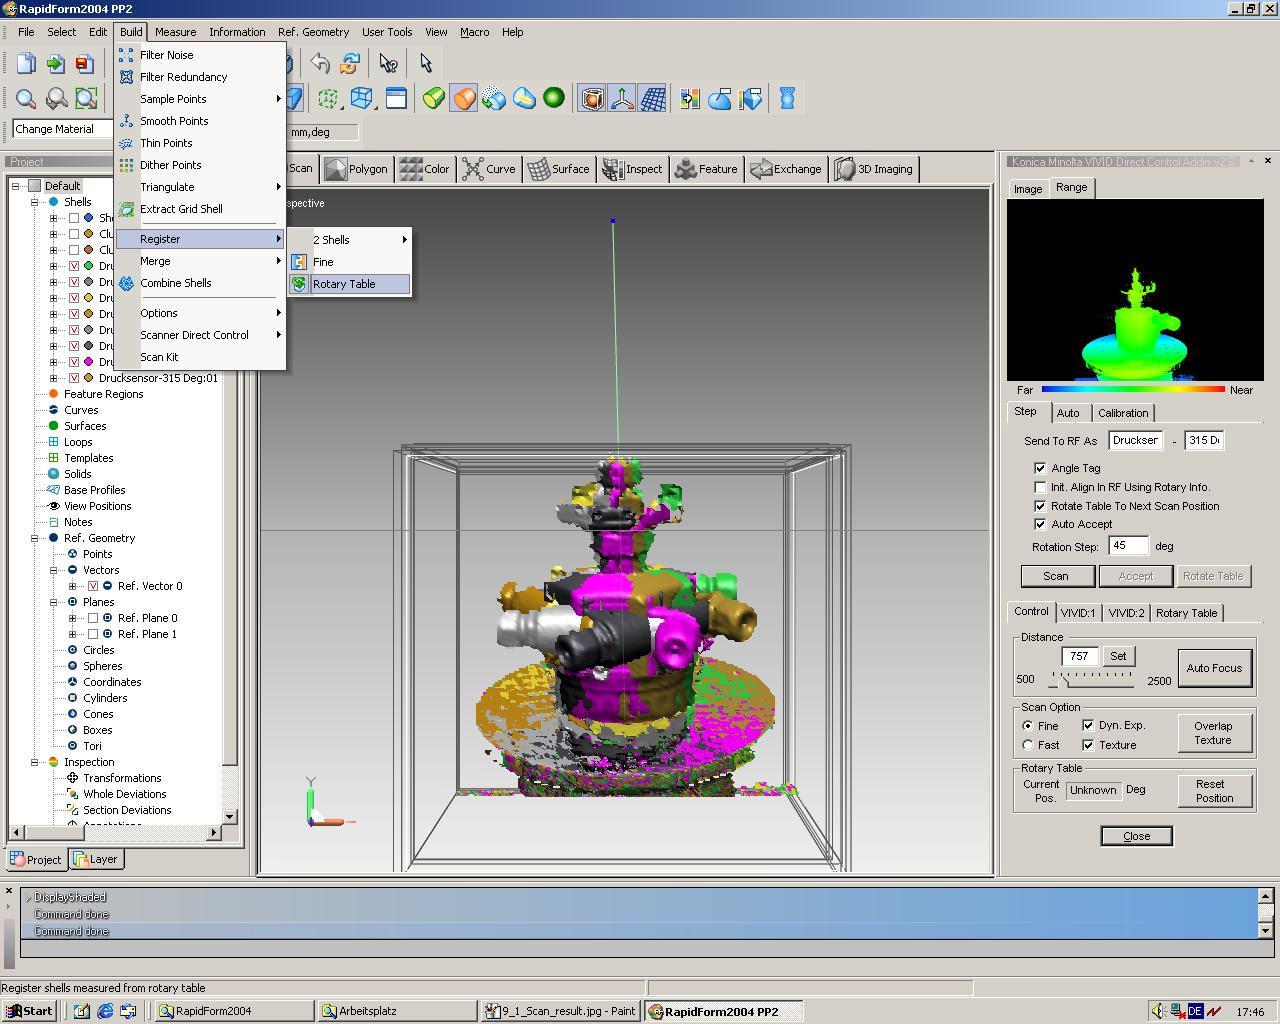
\includegraphics[width=8cm]{Anleitung/10_Rotary_Table}
\\ \hline  

\multicolumn{2}{|l|}%
{{\textbf{Schritt 18 - Registrieren}}}
\\ \hline
Im Dialog auf \textbf{Select Axis} klicken.\linebreak
Im Darstellungsbereich auf die Achse aus dem Kalibrationsscan klicken.
Bei \textbf{Rotation-Angle} den Winkel eines Scans eintragen.\linebreak
Im \emph{Projektbaum} den Entsprechenden Scan auswählen.\linebreak
Die letzten beiden Schritte mit allen Scans wiederholen.\linebreak
Den Dialog mit \textbf{Ok} verlassen.
& 
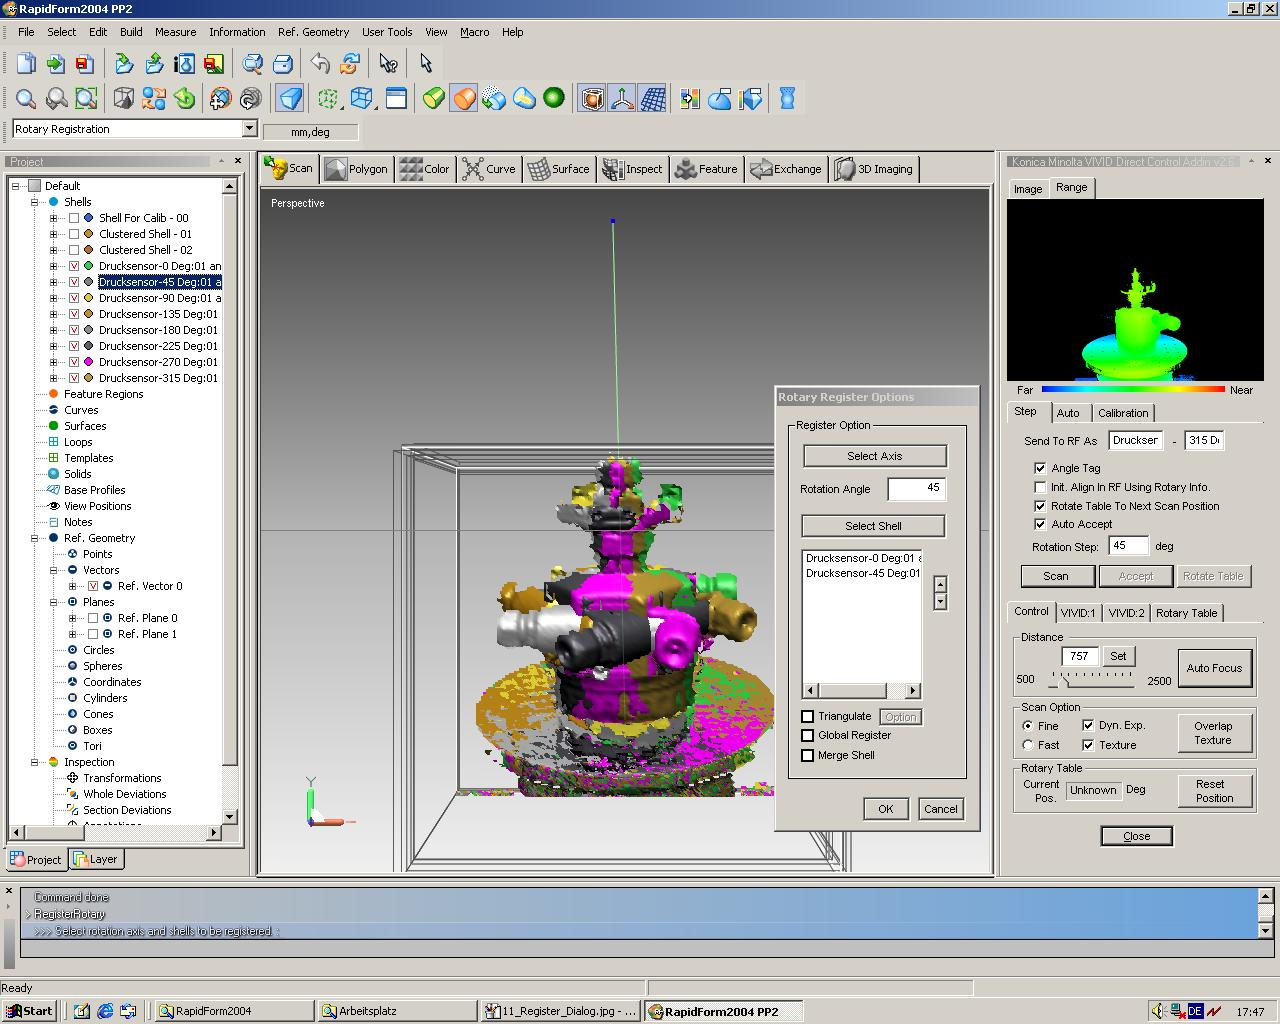
\includegraphics[width=8cm]{Anleitung/11_Register_Dialog_2}
\\ \hline  

\pagebreak

\multicolumn{2}{|l|}%
{{\textbf{Schritt 19 - Ergebnis}}}
\\ \hline
Das Ergebnis ist ein komplettes 3D-Modell des Objektes.
& 
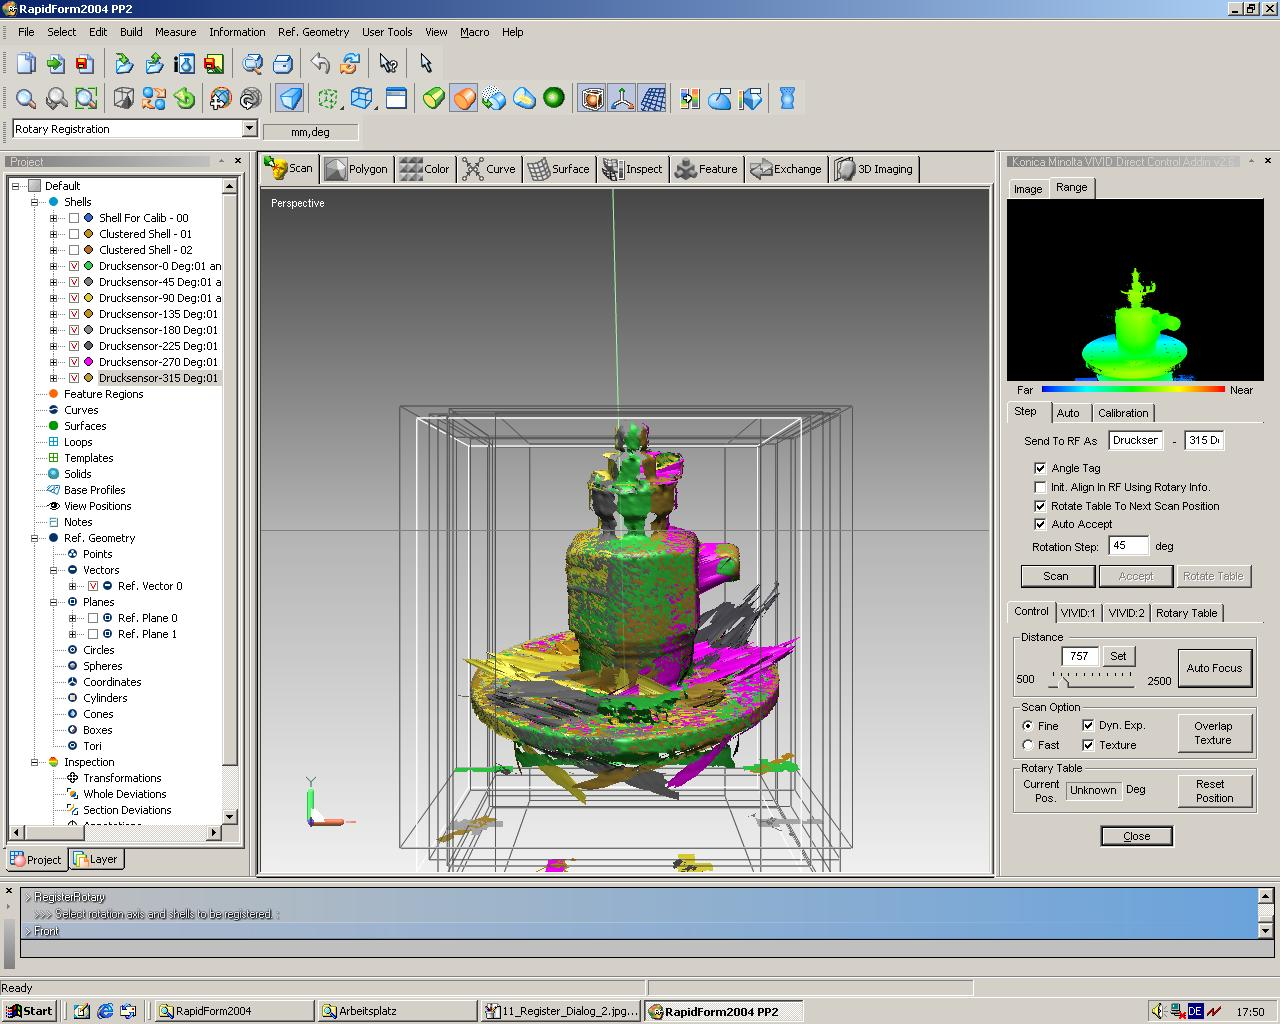
\includegraphics[width=8cm]{Anleitung/11_Register_result}
\\ \hline  

\end{longtable} 